\section{Data Vault}
Our chosen storage format for the data is a data vault~\cite{Linstedt2015}. It allows for new sources of data to be added without the need for a complex redesign of the existing data structures. Additionally, it places an emphasis on data lineage and provenance, ensuring accountability is maintained for any processes taking place on the platform. 

Both the flexibility to accommodate change, and the emphasis on recording the data's journey, will be important factors as more data sets are combined from health services around the world. The ability to consume massively different styles, schemas, and formats of source data, bring them into a single format, and ensure accountability for this transformation is vital as part of any platform wishing to be both powerful, and transparent.

The structure of a data vault relies on three component table types. These are:
\begin{itemize}
    \item Hubs - carries the business keys of the data set
    \item Links - joins the hubs together
    \item Satellites - joined to the hubs and carries the descriptive data in small tables, each one containing only very closely related data
\end{itemize}

\begin{figure}[H]
    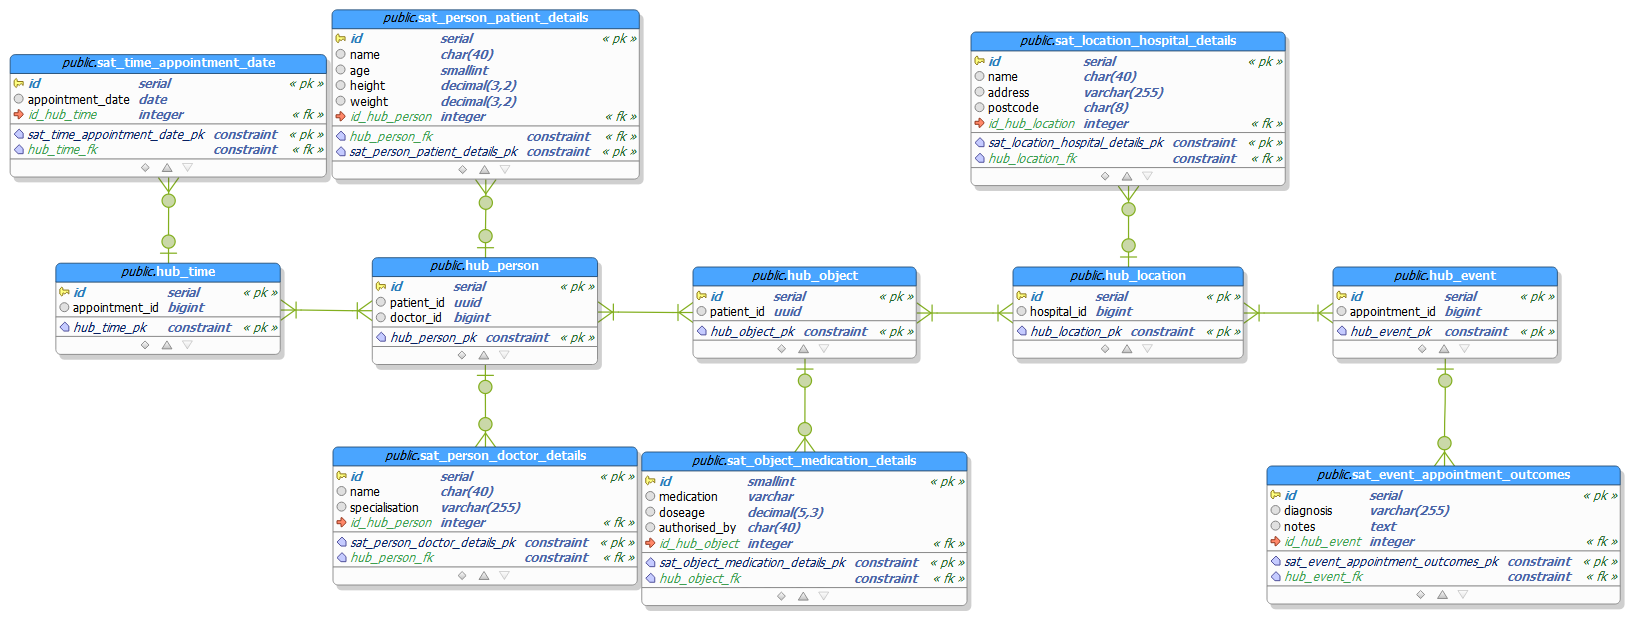
\includegraphics[width=12cm]{images/tpole_plus_sats.png}
    \caption{An example data vault. Hubs form the backbone with Satellites carrying the descriptive details} 
    \label{fig:tpole_sats}
\end{figure}

The Hubs form the backbone of the data vault structure and are used to categorise the data. For our purposes, we have chosen Time, Person, Object, Location, and Event (TPOLE). With these five categories, we are able to classify any of the incoming data. 

With a category assigned to each new piece of data, it is then evaluated as to whether it is closely related enough to the contents of any existing Satellite, under the same category. If it is closely enough related, it will be added to that Satellite, otherwise it will be placed in a new one. This process can be repeated at any stage, whenever a new data source is identified without the destruction of any of the existing data within the data vault.

The trade-off for this flexibility is the need to understand the incoming data. Currently this is a manual process in the Serums \cite{janjic2019serums} project, however plans are in place to introduce elements of machine learning in order to speed this up.

For our Covid-19 project we used a simple rules engine that forms a weak AI to match the data into the T-P-O-L-E categories that then directly mapped into one of the hubs of the data vault.
